%
% Risch-Algorithmus für logarithmische Erweiterungen
%
\subsection{Risch-Algorithmus für logarithmische Erweiterungen
\label{buch:intalg:risch:logarithmisch}}
Im vorangegangenen Abschnitt wurde die Vorgehensweise des Algorithmus
skizziert.
Einzelne Punkte blieben dabei offen, zum Beispiel hing die Durchführbarkeit
der Methode von Hermite davon ab, ob $b(\vartheta)$ und $Db(\vartheta)$
teilerfremd sind.
Das Integral des polynomiellen Teils blieb völlig offen.
In diesem Abschnitt sollen diese Lücken für den Fall einer logarithmischen
Erweiterung geschlossen werden.
Im Folgenden ist $\vartheta=\log u$ also ein Logarithmus,
es gilt $D\vartheta = Du/u$.

%
% Hermite-Methode
%
\subsubsection{Hermite-Methode}
Für eine logarithmische Erweiterung ist $D\vartheta=Du/u$.
Für ein Polynom $b(\vartheta)$ folgt dann
\begin{align*}
Db(\vartheta)
&=
\sum_{k=0}^m
Db_k\vartheta^k
+
\sum_{k=0}^m
b_k k
\frac{Du}{u}
\vartheta^{k-1}.
\end{align*}
Wegen $Du\in F$ sind die Koeffizienten $Db_k$ und $kb_kDu/u\in F$,
$Db(\vartheta)$ ist also wieder ein Polynom in $F[\vartheta]$ vom
gleichen Grad wie $b(\vartheta)$.
Die Polynome $Db(\vartheta)$ und $b'(\vartheta)$ unterscheiden sich
damit deutlich.
Trotzdem zeigt das nachfolgende Lemma, dass für eine logarithmische 
Erweiterung $Db(\vartheta)$ und $b(\vartheta)$
teilerfremd sind, wenn $b(\vartheta)$ und $b'(\vartheta)$ teilerfremd sind.

\begin{lemma}
\label{buch:intalg:risch:log:lemma:bDb}
Sei $b(\vartheta)$ ein normiertes, quadratfreies Polynom mit
$b(\vartheta)$ und $b'(\vartheta)$ teilerfremd als Polynome in $F[\vartheta]$,
dann sind auch $b(\vartheta)$ und $Db(\vartheta)$ teilerfremd.
\end{lemma}

\begin{proof}
Da es in diesem Lemma nicht um einen Teil des Algorithmus geht, sondern
um eine Teilbarkeitseigenschaft der Polynome, dürfen wir für den Beweis
nach dem Fundamentalsatz der Algebra annehmen, dass wir eine Faktorisierung
\begin{equation}
b(\vartheta)
=
\prod_{i=1}^m (\vartheta-\beta_i)
\label{buch:ointalg:risch:log:eqn:bfaktorisierung}
\end{equation}
in Linearfaktoren kennen.
Ihre Ableitung ist
\begin{align}
Db(\vartheta)
&=
\sum_{k=1}^m D(\vartheta-\beta_k)\prod_{i\ne k} (\vartheta-\beta_i)
\notag
\\
&=
\sum_{k=1}^m \biggl(\frac{Du}{u}-D\beta_k\biggr)
\prod_{i\ne k} (\vartheta-\beta_i).
\label{buch:intalg:risch:log:eqn:Dbfaktorisierung}
\end{align}
Weil $b(\vartheta)$ und $b'(\vartheta)$ teilerfremd sind, dürfen wir
davon ausgehen, dass die $\beta_i$ alle verschieden sind, sie sind alle
einfache Nullstellen.

Wir müssen zeigen, dass auch $b(\vartheta)$ und $Db(\vartheta)$ keinen
nichtrivialen gemeinsamen Teiler haben können.
Ein gemeinsamer Linearfaktor von $b(\vartheta)$ und $Db(\vartheta)$
muss einer der Faktoren von \eqref{buch:ointalg:risch:log:eqn:bfaktorisierung}
sein, sei $\vartheta-\beta_j$ dieser Faktor.
$\vartheta-\beta_j$ kommt in jedem Term auf der rechten Seite von
\eqref{buch:intalg:risch:log:eqn:Dbfaktorisierung} ausser möglicherweise
im Term $k=j$ vor.
Er teilt daher jeden Term ausser möglicherweise $k=j$.
Da $\vartheta-\beta_j$ ein Teiler der ganzen Gleichung sein muss,
im Produktfaktor für $k=j$ aber nicht vorkommt,
muss $\vartheta-\beta_j$ auch den Faktor $Du/u-D\beta_j$ teilen.
In $Du/u-D\beta_j$ kommt $\vartheta$ nicht vor, es ist ein Polynom vom
Grad $0$, welches von einem Polynom $\vartheta-\beta_j$ vom Grad 1
geteilt wird.
Dies ist nur möglich, wenn
\[
D(\vartheta-\beta_j) = 0
\qquad\Rightarrow\qquad
\vartheta-\beta_j = c,\; c\in K
\qquad\Rightarrow\qquad
\vartheta = \beta_j+ c \in F
\]
ist.
Dies widerspricht der Tatsache, dass $\vartheta$ eine transzendente
Erweiterung von $F$ ist.
\end{proof}

Lemma~\ref{buch:intalg:risch:log:lemma:bDb} zeigt, dass die Methode
von Hermite uneingeschränkt durchführbar ist.

%
% Der Beweis von Lemma 8.26
%
\subsubsection{Der Beweis von Lemma~\ref{buch:intalg:risch:lemma:v0log}}
\begin{proof}[Beweis von von Lemma~\ref{buch:intalg:risch:lemma:v0log}]
Wegen $v_0(\vartheta)\in F(\vartheta)$
dürfen wir annehmen, dass
\[
v_0(\vartheta)
=
\frac{p(\vartheta)}{q(\vartheta)}
\]
ist mit teilerfremden Polynomen $p(\vartheta),q(\vartheta)\in F[\vartheta]$
und $q(\vartheta)$ normiert.
Für eine logarithmische Ableitung ist nach
Satz~\ref{buch:intalg:liouville:polynome:satz:logarithmisch}
die Ableitung eines Polynoms in $F[\vartheta]$ wieder ein Polynom
in $F[\vartheta]$ und die Ableitung eines normierten Polynoms ist
von kleinerem Grad:
$\deg Dq(\vartheta)<\deg q(\vartheta)$.
Die Ableitung von $v_0(\vartheta)$ ist dann
\begin{equation}
Dv_0(\vartheta)
=
\frac{
Dp(\vartheta)\cdot q(\vartheta) - p(\vartheta)\cdot Dq(\vartheta)
}{
q(\vartheta)^2
}
=
\frac{ Dp(\vartheta) }{ q(\vartheta) }
-
\frac{p(\vartheta)}{q(\vartheta)}\cdot\frac{Dq(\vartheta)}{q(\vartheta)}
\label{buch:intalg:risch:eqn:Dv0}
\end{equation}
Selbst wenn $Dq(\vartheta)$ und $q(\vartheta)$ einen gemeinsamen Faktor haben,
bleibt immer noch ein Faktor vom Grad mindestens 1 im Nenner
des letzten Bruchs von \eqref{buch:intalg:risch:eqn:Dv0}, der gegen
den Zähler $Dq(\vartheta)$ nicht gekürzt werden kann und daher im Nenner
des zweiten Terms zweimal vorkommt.
Somit ist der Nenner des zweiten Terms nicht quadratfrei.
Da aber alle anderen Terme in
\eqref{buch:intalg:risch:rt:eqn:liouvillediff}
quadratfreien Nenner haben, muss auch $Dv_0(\vartheta)$ quadratfreien
Nenner haben, es folgt $q(\vartheta)=1$.

Sei jetzt also $\deg p(\vartheta)\ge 1$.
Der Grad der Ableitung ist dann
$\deg Dv_0(\vartheta) = \deg Dp(\vartheta) \ge 0$.
Macht man alle Terme in 
\eqref{buch:intalg:risch:rt:eqn:liouvillediff}
gleichnamig, entsteht im Zähler der rechten Seite wegen dem Summanden
$v_0(\vartheta)$ ein Zähler vom Grad, der mindestens so gross ist
wie der Nennergrad.
Auf der linken Seite ist der Zählergrad aber nach Voraussetzung 
kleiner als der Nennergrad.
Dieser Widerspruch zeigt, dass $v_0(\vartheta)=0$ sein muss.
\end{proof}

%
% Rothstein-Trager für logarithmische Erweiterungen
%
\subsubsection{Rothstein-Trager für logarithmische Erweiterungen}
Die Methode von Rothstein-Trager bestimmt die Stammfunktion eines
rationalen Teils $a(\vartheta)/b(\vartheta)$ aus den Elemente
$c_k$ und $v_k(\vartheta)$, die in
Satz~\ref{buch:intalg:risch:satz:rothstein-trager-allgemein}
definiert worden sind.
In der Tat wurde im Beweis jenes Satzes auch schon fast alles
bewiesen, was der folgende Satz besagt.

\begin{satz}[Rothstein-Trager]
\label{buch:intalg:risch:satz:rothstein-trager-logarithmisch}
Sei $F\subset F(\vartheta)$ eine logarithmische Erweiterung und 
\[
f = \frac{a(\vartheta)}{b(\vartheta)}
\]
ein rationaler Teil.
Dann gilt:
\begin{enumerate}
\item
$f$ hat eine elementare Stammfunktion genau dann, wenn die 
Elemente $c\in F$, für die 
\[
a(\vartheta) - c \cdot Db(\vartheta)
\qquad\text{und}\qquad
b(\vartheta)
\]
einen nichttrivialen gemeinsamen Teiler haben, Konstanten $c_k\in K$,
$k=1,\dots,m$ sind.
\item
Hat $f$ eine elementare Stammfunktion, dann ist sie
\begin{equation}
\int f
=
\int \frac{a(\vartheta)}{b(\vartheta)}
=
\sum_{k=1}^m c_i \log v_k(\vartheta).
\label{buch:intalg:risch:satz:rtlog:summe}
\end{equation}
\end{enumerate}
\end{satz}

\begin{proof}
Die einzige, im Beweis von
Satz~\ref{buch:intalg:risch:satz:rothstein-trager-allgemein}
noch nicht bewiesen Aussage ist, dass die Summe
\eqref{buch:intalg:risch:satz:rtlog:summe}
die Stammfunktion ist.
Wir schreiben daher
\[
\bar{a}(\vartheta)
=
\sum_{k=1}^m b(\vartheta) c_k \frac{Dv_k(\vartheta)}{v_k(\vartheta)}
=
\sum_{k=1}^m c_k Dv_k(\vartheta) u_k(\vartheta)
\qquad\text{mit}\qquad
u_k(\vartheta) = \frac{b(\vartheta)}{v_k(\vartheta)}
=
\prod_{\scriptstyle i=1 \atop\scriptstyle i\ne k}^m v_i(\vartheta)
\]
Die gesuchte Aussage ist dann äquivalent dazu, dass
$a(\vartheta)=\bar{a}(\vartheta)$ ist.
Für alle $k$ gilt
\[
\bar{a}(\vartheta) - c_k Db(\vartheta)
=
\sum_{i=1}^m (c_i-c_k)Dv_i(\vartheta)u_i(\vartheta).
\]
Der Summand $i=k$ verschwindet auf der rechten Seite, alle
anderen Summanden haben $v_k(\vartheta)$ als Teiler, da
$v_k(\vartheta)\mid u_i(\vartheta)$ für $i\ne k$.
Somit ist $v_k(\vartheta)$ ein gemeinsamer Teiler von
$\bar{a}(\vartheta)-c_kDb(\vartheta)$ und $b(\vartheta)$.

Nach Definition von $v_k(\vartheta)$ ist $v_k(\vartheta)$ auch ein
Teiler von $a(\vartheta)-c_kDb(\vartheta)$.
Aus
\begin{align*}
v_k(\vartheta)&\mid (\bar{a}(\vartheta)-c_kDb(\vartheta))\\
v_k(\vartheta)&\mid (a(\vartheta)-c_kDb(\vartheta))
\end{align*}
folgt aber auch, dass $v_k(\vartheta)\mid (\bar{a}(\vartheta)-a(\vartheta))$
ist.
Da die $v_k(\vartheta)$ teilerfremd sind, ist auch deren Produkt
$b(\vartheta)$ ein Teiler von $\bar{a}(\vartheta)-a(\vartheta)$.

Nach Voraussetzung ist $\deg a(\vartheta)<\deg b(\vartheta)$.
Da $\vartheta$ ein Logarithmus ist, ist nach
Satz~\ref{buch:intalg:liouville:polynome:satz:logarithmisch}
auch
$\deg Dv_k(\vartheta) < \deg v_k(\vartheta)$ und
$\deg b(\vartheta) < \deg b(\vartheta)$ (an dieser Stelle wird
gebraucht, dass die Erweiterung $\vartheta$ logarithmisch ist).
Somit ist auch $\deg \bar{a}(\vartheta) < \deg b(\vartheta)$ und daher
auch $\deg (\bar{a}(\vartheta)-a(\vartheta)) < \deg b(\vartheta)$.
$b(\vartheta)$ kann aber nur Teiler eines Polynoms kleineren Grades sein,
wenn dieses Polynom das Nullpolynom ist.
Somit ist $\bar{a}(\vartheta)=a(\vartheta)$ und damit ist der
Satz beweisen.
\end{proof}

Nachfolgend wird an zwei Beispielen gezeigt, wie die Stammfunktion mit
der Methode von Rothstein-Trager gefunden werden kann.
Die Beispiele sind einfach genug, dass man Teilbarkeit ad hoc untersuchen
kann.
Eine systematischere Vorgehensweise verwendet die Resultante und wird
in Kapitel~\ref{chapter:resultante} dargestellt.

\begin{beispiel}
\label{buch:intalg:risch:bsp:1/logx}
Hat die Funktion
\[
f(x)
=
\frac{1}{\log x}
\]
eine elementare Stammfunktion?
\medskip

Der Integrand liegt in der logarithmischen Erweiterung
$F(\vartheta) = \mathbb{Q}(x,\log x)$ von $F=\mathbb{Q}(x)$
um das logarithmische Element $\vartheta=\log x$.
$f(x)$ hat nur den rationalen Teil
\[
f(x)
=
\frac{1}{\vartheta}
\qquad
\Rightarrow
\qquad
\begin{cases}
a(\vartheta) &= 1 \\
b(\vartheta) &= \vartheta.
\end{cases}
\]
Dies ist bereits die Ausgangsform für die Methode von Rothstein-Trager,
die verlangt, dass die Werte von $z$ bestimmt werden müssen, für die
die beiden Polynome
\[
a(\vartheta) - z\cdot Db(\vartheta)
1 - z\,D\vartheta
=
1- z\frac{1}{x}
\qquad\text{und}\qquad
b(\vartheta)=\vartheta
\]
gemeinsame Teiler haben.
Da das linke Polynom Grad 0 hat, kann es nur dann ein Polynom vom Grad
mindestens $1$ als Teiler haben, wenn es verschwindet.
Die Bedinungung für gemeinsame Teiler ist daher
\[
1-z\frac{1}{x} = 0 
\qquad\Rightarrow\qquad
z=x,
\]
insbesondere ist $z$ nicht konstant.
Es folgt, dass $f$ kein elementare Stammfunktion hat.
\end{beispiel}

Im Beispiel wurde bewiesen, dass $1/\log x$ keine elementare Stammfunktion
hat.
Das Integral hat aber einige Bedeutung in der analytischen Zahlentheorie,
da sie ein Approximation für die Primzahlzählfunktion 
\[
\pi(x)
=
\bigl|
\{ p \mid \text{$p$ ist prim und $p\le x$} \}
\bigr|
\]
ist.
Es bleibt daher nichts anderes übrig, als eine neue spezielle Funktion
dafür zu definieren.

\begin{definition}[Integrallogarithmus]
\label{buch:intalg:risch:def:integrallogarithmus}
%
% fig-li.tex -- Graph der Funktion li(x)
%
% (c) 2026 Prof Dr Andreas Müller
%
\begin{figure}
\centering
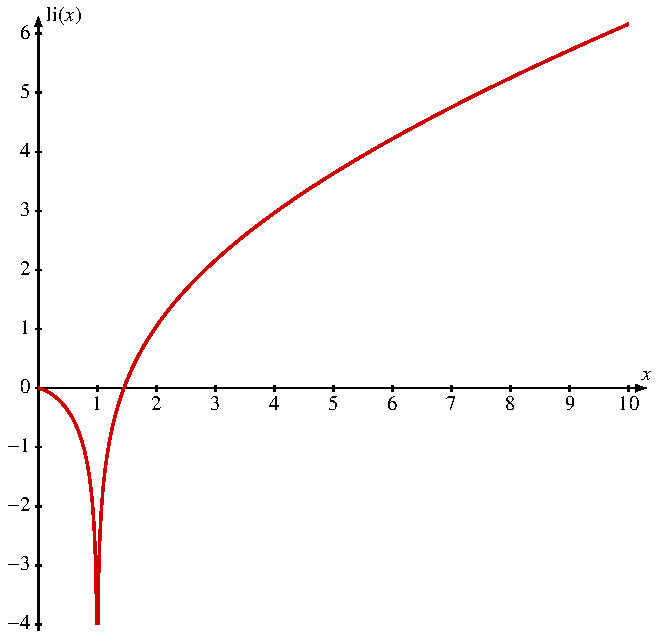
\includegraphics{chapters/070-intalg/images/li.pdf}
\caption{Graph der Integrallogarithmusfunktion
$\operatorname{li}(x)$ für $x>0$.
\label{buch:intalg:fig:li}}
\end{figure}
%
Das bestimmte Integral
\[
\operatorname{li}(x)
=
\int_0^x
\frac{1}{\log t}
\,dt
\]
heisst der \emph{Integrallogarithmus}.
\index{Integrallogarithmus}%
\index{li(x)@$\operatorname{li}(x)$}%
\end{definition}

Eine graphische Darstellung des Graphen von $\operatorname{li}(x)$ ist
in Abbildung~\ref{buch:intalg:fig:li} wiedergegeben.
Da der Integrand an der Stelle $x=1$ eine Singularität hat, muss dieser
Argumentwert mit dem Hauptwert überbrückt werden.
Die Funktion ist daher für $x>1$ durch
\[
\operatorname{li}(x)
=
\lim_{\varepsilon\to 0+}
\biggl(
\int_0^{1-\varepsilon} \frac{dt}{\log t}
+
\int_{1+\varepsilon}^x \frac{dt}{\log t}
\biggr)
\]
definiert.

\begin{beispiel}
Hat die Funktion $1/x\log x \in \mathbb{Q}(x,\log x)$ eine elementare
Stammfunktion?
Mit $\vartheta=\log x$ ist die Stammfunktion des rationalen Teils
\begin{equation}
\frac{1}{x\vartheta}
=
\frac{1/x}{\vartheta}
=
\frac{a(\vartheta)}{b(\vartheta)}
\qquad\Rightarrow\qquad
\begin{cases}
a(\vartheta) &= 1/x\\
b(\vartheta) &= \vartheta
\end{cases}
\label{buch:intalg:risch:eqn:1xlogx}
\end{equation}
nach der Methode von Rothstein-Trager zu bestimmen.
Dazu müssen gemeinsame Teiler von
\[
a(\vartheta) - z\cdot Db(\vartheta)
=
\frac{1}{x} - zD\vartheta
=
\frac{1}{x} - z\frac{1}{x}
\qquad\text{und}\qquad
b(\vartheta)=\vartheta
\]
bestimmt werden.
Da das linke Polynom Grad 0 hat, kann es nur dann nichttriviale
Teiler vom Grad mindestens 1 geben, wenn es verschwindet, wenn also
\[
\frac{1}{x} - z\frac{1}{x}
=
0
\qquad\Rightarrow\qquad
\frac{1-z}{x}
=
0
\qquad\Rightarrow\qquad
c=z=1.
\]
Der gemeinsame Teiler ist $v=\vartheta=\log x$.
Nach der Methode von Rothstein-Trager ist daher
\[
f(x)
=
1\frac{Dv}{v}
=
\frac{1}{x \vartheta}
\qquad\Rightarrow\qquad
\int f
=
\log v
=
\log \vartheta
=
\log\log x,
\]
ein elementare Stammfunktion des Integranden $f$.

Die Wahl $a(\vartheta)=1/x$ in \eqref{buch:intalg:risch:eqn:1xlogx}
wird dadurch festgelegt, dass $b(\vartheta)$ ein normiertes Polynom
sein muss.
Der Faktor $x$ im Nenner von \eqref{buch:intalg:risch:eqn:1xlogx}
kann daher nicht Teil des Polynoms $b(\vartheta)$ sein, sondern muss
in $a(\vartheta)$ integriert werden.
\end{beispiel}

%
% Der polynomielle Teil für logarithmische Erweiterungen
%
\subsubsection{Der polynomielle Teil für logarithmische Erweiterungen}
Wir betrachten wieder die Situation einer logarithmischen Erweiterung
$F(\vartheta)\supset F$ um ein logarithmisches Element $\vartheta =\log u$
mit Konstantenkörper $K$.
Wir versuchen die Stammfunktion des polynomiellen Teils in $F(\vartheta)$
zu bestimmen, den wir als
\begin{equation}
p(\vartheta)
=
p_0 + p_1\vartheta + \dots + p_{l-1}\vartheta^{l-1} + p_l\vartheta^l
\in
F[\vartheta]
\label{buch:intalg:risch:eqn:logpolyintegrand}
\end{equation}
schreiben.
Für ein Polynom in der unabhängigen Variablen $x$ ist die Stammfunktion
trivialerweise elementar, da 
\[
\int p_kx^k \,dx = \frac{p_k}{k+1}z^{k+1} + C
\]
ist.
Dies funktioniert jedoch nur für konstante Koeffizienten.
In der vorliegenden allgemeinen Situation
\eqref{buch:intalg:risch:eqn:logpolyintegrand}
erwarten wir eine wesentlich kompliziertere Lösung.

Falls $p(\vartheta)$ eine elementare Stammfunktion hat, dann muss 
sie nach dem Liouville-Prinzip die Form
\begin{align}
\int p(\vartheta)
&=
v_0(\vartheta) + \sum_{i=1}^n c_i\log v_i(\vartheta)
\notag
\intertext{mit $v_i(\vartheta) \in F(\vartheta)$ und $c_i\in K$ haben.
Wie früher darf man annehmen, dass die $v_i(\vartheta)$ teilerfremde,
quadratfreie Polynome sind.
In der abgeleiteten Form ist}
p(\vartheta)
&=
Dv_0(\vartheta)
+
\sum_{i=1}^n c_i \frac{Dv_i(\vartheta)}{v_i(\vartheta)}.
\notag
\intertext{Auf der linken Seite dieser Gleichung steht ein Polynom,
auf der rechten Seite kommen die Nenner $v_i(\vartheta)$ vor.
Da sie teilerfremd sind, können sich die Brüche nicht wegheben, in den
Termen der Summe darf also $\vartheta$ gar nicht vorkommen.
Es bleibt daher die Form}
p(\vartheta)
&=
Dq(\vartheta) + \sum_{i=1}^n c_i \frac{Dv_i}{v_i}
\notag
\\
&=
D(q_{l+1}\vartheta^{l+1} + q_l\vartheta^l + \dots + q_2\vartheta^2
+ q_1\vartheta) + Dq_0 + \sum_{i=1}^n c_i\frac{Dv_i}{v_i}
\label{buch:intalg:risch:logarithmisch:eqn:pDq}
\end{align}
mit $v_i\in F$, $c_i\in K$ und $q\in F[\vartheta]$.
Die Aufgabe ist, das Polynom $q(\vartheta)$ zu bestimmen.

Der Koeffizient $q_0$ für sich alleine interessiert nicht wirklich,
da für die gesuchte Stammfunktion nur die Kombination
\[
\bar{q}_0
=
q_0 + \sum_{i=1}^n c_i\log v_i
\]
benötigt wird.

Zur Bestimmung der Koeffizienten $q_k$ und $\bar{q}_0$ vergleichen wir
Koeffizienten in 
\eqref{buch:intalg:risch:logarithmisch:eqn:pDq}.
Es ergeben sich die Gleichungen
\begin{align*}
0   &= Dq_{l+1}
	&&\Rightarrow
	& Dq_{l+1} &= 0
\\[-4pt]
p_l &= Dq_l + q_{l+1}(l+1) \frac{Du}{u}
	&&\Rightarrow
	& Dq_l     &= p_l - (l+1)q_{l+1}\frac{Du}{u}
\\[-9pt]
    &\phantom{n}\vdots 
	&&           &
	&\phantom{n}\vdots
\\[-9pt]
p_k &= Dq_k + q_{k+1}(k+1) \frac{Du}{u}
	&&\Rightarrow
	& Dq_k     &= p_k - (k+1)q_{k+1}\frac{Du}{u}
\\[-9pt]
    &\phantom{n}\vdots        
	&&
	&          &\phantom{n}\vdots
\\[-9pt]
p_1 &= Dq_1 + 2q_2 \frac{Du}{u}
	&&\Rightarrow
	& Dq_1     &= p_1 - 2q_2 \frac{Du}{u}
\\[-0pt]
p_0 &= D\bar{q}_0 + q_1 \frac{Du}{u}
	&&\Rightarrow& D\bar{q}_0 &= p_1 - q_1 \frac{Du}{u}
\end{align*}
Die rechten Seiten zeigen, dass alle Koeffizieten von $q(\vartheta)$
als Lösung eines Integrationsproblems im kleineren Körper $F$ gefunden
werden müssen.
Jedes dieser einzelnen Integrationsproblem muss eine elementare
Lösung in $F(\vartheta)$ haben.
Die Lösung des Integrationsproblems für $d_k$ ist aber immer nur bis auf
eine Integrationskonstante $b_k$ bestimmt.

Aus der ersten Gleichung folgt, dass $q_{l+1}$ eine Konstante sein muss,
die mit $b_{l+1}$ bezeichnet wird.
Da $q_{l+1}$ auch in der Gleichung für $q_l$ auftritt, kann
letztere zur Bestimmung von $b_{l+1}$ herangezogen werden.

Die Gleichung für $q_l$ wird mit der Lösung für $q_{l+1}$ zu
\[
Dq_l
=
p_l-(l+1)b_{l+1}\frac{Du}{u}.
\]
Die Lösung muss eine elementare Funktion sein, nach dem Prinzip von Liouville
muss
\[
q_l
=
d_l + c_l\vartheta + b_l
\]
mit $d_l\in F$ und $c_l,b_l\in K$ sein.
Durch Ableiten und Vergleich mit der Gleichung für $Dq_l$ schilessen wir,
dass
\[
p_l - (l+1)b_{l+1}\frac{Du}{u} 
=
Dq_l 
=
Dd_l + c_l\frac{Du}{u}
\qquad\Rightarrow\qquad
\left\{
\;
\renewcommand{\arraycolsep}{2pt}
\begin{array}{rcl}
\displaystyle d_l     &=& \displaystyle \int p_l \\[9pt]
\displaystyle b_{l+1} &=& \displaystyle -\frac{c_{l}}{l+1}.
\end{array}
\right.
\]
sein muss.
Damit ist jetzt auch die Integrationskonstante $b_{l+1}$ bestimmt.

Nehmen wir an, dass die Koeffizienten bis $q_{k+1} = d_{k+1}+b_{k+1}$
bereits bestimmt sind.
Nur die Integrationskonstante $b_{k+1}$ ist noch zu bestimmen.
Die Bestimmungsgleichung
\begin{align*}
Dq_k &= p_k - (k+1) q_{k+1} \frac{Du}{u}
\intertext{wird damit zu}
Dq_k
&=
p_k
-
(k+1) d_{k+1} \frac{Du}{u}
-
(k+1) b_{k+1} \frac{Du}{u}.
\intertext{Der letzte Term kann ist sofort integrierbar, wir können
daher die Terme so sortieren, dass}
p_k
-
(k+1) d_{k+1} \frac{Du}{u}
&=
Dq_k
+
(k+1) b_{k+1} \frac{Du}{u}.
\end{align*}
Die linke Seite muss also eine elementare Stammfunktion haben,
die nach dem Prinzip von Liouville wieder in der Form $d_k + c_k\vartheta$
geschrieben werden kann.
Durch Ableiten und Termvergleich können wir wieder
\[
\left.
\renewcommand{\arraycolsep}{2pt}
\begin{array}{rcl}
d_k
&=&
\displaystyle
\int\biggl(
p_k
-
(k+1) d_{k+1} \frac{Du}{u}
\biggr)
\\[9pt]
b_{k+1}
&=&
\displaystyle
-
\frac{c_k}{k+1}
\end{array}
\;
\right\}
\quad\Rightarrow\quad
q_k = d_k + b_k
\]
schliessen.
Dieser Schritt kann für kleiner werdende $k$ wiederholt werden bis
$q_1=d_1+b_1$ bsetimmt ist, wobei die Integrationskonstante $b_1$ noch
zu finden ist.

%
% polylog.tex
%
% (c) 2026 Prof Dr Andreas müller
%
\begin{figure}
\centering
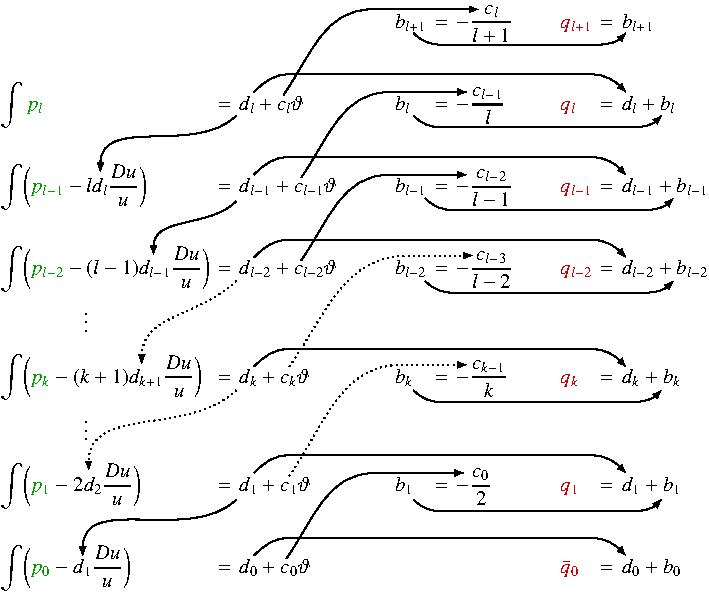
\includegraphics{chapters/070-intalg/images/polylog.pdf}
\caption{Gang der Rechnung für den polynomiellen Teil im Fall einer
logarithmischen Erweiterung.
Aus den bekannten Koeffizienten $p_k\in F$ wird zunächst der Integrand
gebildet, wozu $d_{k-1}$ aus dem vorangegangenen Schritt benötigt wird.
Die Stammfunktion liefert $d_k$ und die Konstante $c_k$, mit der sich
die Integrationskonstaten $b_{k-1}$ im vorangegangenen Schritt
festlegen lässt.
\label{buch:intalg:risch:logarithmisch:fig:polylog}}
\end{figure}
%

Die Bestimmungsgleichung für $\bar{q}_0$ ist
\[
D\bar{q}_0
=
p_0 - q_1\frac{Du}{u}
=
p_0 - d_1\frac{Du}{u} - c_1\frac{Du}{u}
\quad\Rightarrow\quad
D\bar{q}_0
-
c_1\frac{Du}{u}
=
p_0 - d_1\frac{Du}{u}.
\]
Um $\bar{q}_0$ zu bestimmen, muss eine Stammfunktion gefunden werden.
Dazu muss wieder das Integrationsproblem für den Integranden ganz rechts
gelöst werden.
Im Gegensatz zu den früheren Schritten darf die Stammfunktion
\[
\int
\biggl(
p_0 - d_1\frac{Du}{u}
\biggr)
=
d_0
=
v_0 + \sum_{i=1}^m \bar{c}_i \log v_i, \qquad \bar{c}_i\in K
\]
aber auch andere Logarithmen als $\vartheta$ enthalten, solange
sie Logarithmen von Elemente von $F$ sind.
Einer der Logarithmen darf $\vartheta$ sein, sei dies der erste.
Aus der Konstanten $\bar{c}_1$ lässt sich dann auch auch
\(
b_1 = -\bar{c}_1
\)
bestimmen.
Dadurch ist $\bar{q}_0=d_0$ jetzt bis auf eine Konstante unbekannte
Integrationskonstante $b_0$ bestimmt.

Der Gang der Berechnung ist in
Abbildung~\ref{buch:intalg:risch:logarithmisch:fig:polylog} 
schematisch dargestellt.
Im Schritt zur Bestimmung von $q_k$ wird zunächst aus dem bekannten
Koeffizienten $p_k$ und der Stammfunktion $d_{k-1}$ aus dem vorangegangenen
Schritt der Integrand gebildet.
Seine Stammfunktion liefert $d_k$ und die Konsante $c_k$.
Die Integrationskonstante $b_{k-1}$ im vorangegangenen Schritt ist
durch $c_k$ bestimmt.
Schliesslich kann $q_k = d_k+b_k$ gefunden werden.
Nur die letzte Integrationskonstante $b_0$ kann nicht bestimmt werden.

\begin{beispiel}
Man finde die Stammfunktion von $f(x) = \log x$.
Der Integrand ist das Polynom
\[
f(x)=\vartheta
=
1\cdot\vartheta + 0
=
p_1\vartheta + p_0
\qquad\Rightarrow\qquad
\begin{cases}
p_1 &= 1\\
p_0 &= 0.
\end{cases}
\]
in der Erweiterung
$F(\vartheta)=\mathbb{Q}(x,\vartheta)$ von $F=\mathbb{Q}(x)$ um das
logarithmische Element $\vartheta=\log x$.
Es muss also ein Polynom
\[
q(\vartheta)
=
q_2\vartheta^2 + q_1\vartheta + \bar{q}_0
\]
vom Grad 2 gefunden werden.
\begin{itemize}
\item Fall $k=2$:
$q_2$ muss eine Konstante $b_2$ sein, deren Wert im
nächsten Schritt bestimmt wird.
\item Fall $k=1$:
Zur Bestimmung von $q_1$ muss zunächst die Stammfunktion
von $p_1$ bestimmt werden, sie ist
\[
\int p_1
=
\int 1
=
x + 0\cdot\vartheta
\quad
\Rightarrow
\quad
\left\{
\quad
\renewcommand{\arraycolsep}{2pt}
\begin{array}{rcl}
b_2 &=& \displaystyle -\frac{c_1}{2} \\
d_1 &=& x
\end{array}
\quad
\right\}
\quad
\Rightarrow
\quad
q_1 = x + b_1
\]
Da darin $\vartheta$ nicht vorkommt, folgt $c_1=0$ und daher $b_2=0$.
Die Integrationskonstante $b_1$ wird im nächsten Schritt bestimmt.
\item Fall $k=0$:
Es muss die Stammfunktion von $p_0-d_1\,Du/u$ aus
\[
q_0
=
\int\biggl(p_0-d_1\frac{Du}u\biggr)
=
\int\biggl(0-x\frac{1}{x}\biggr)
=
-
\int 1
=
-x
+
b_0
=
d_0+b_0
\]
bestimmt werden.
Auch hier kann man schliessen, dass $b_1=0$ ist.
\end{itemize}
Aus den drei Fällen lässt sich jetzt die Stammfunktion
\[
\int p(\vartheta)
=
q(\vartheta)
=
q_0 + q_1\vartheta + q_2\vartheta^2
=
-x+b_0 + z\vartheta
=
x\log x - x + b_0
\]
ablesen.
Tatsächlich ist die Ableitung davon
\[
\frac{d}{dx}\bigl( x\log x - x + b_0\bigr)
=
\log x + x \frac 1x - 1
=
\log x.
\]
Wie erwartet kann die Integrationskonstante $b_0$ nicht bestimmt werden.
\end{beispiel}

\begin{beispiel}
Hat der Integrand $\log\log x$ eine elementare Stammfunktion?
Für diese Aufgabe muss der Körper der rationalen Funktionen zweimal
logarithmisch erweitert werden, zunächst um $\vartheta_1=\log x$ und
dann im zweiten Schritt um $\vartheta_2 = \vartheta =\log u = \log\log x$.
Gesucht ist jetzt das Integral des Polynoms
$p(\vartheta) = 1\cdot\vartheta + 0$
mit $p_1=1$ und $p_0=0$.
\begin{itemize}
\item Fall $k=2$:
$q_2$ muss eine Konstante $b_2$ sein, deren Wert im
nächsten Schritt bestimmt wird.
\item Fall $k=1$:
Die Stammfunktion $p_1$ ist
\[
\int p_1
=
\int 1
=
x + 0\cdot \vartheta
\quad
\Rightarrow
\quad
\left\{
\quad
\renewcommand{\arraycolsep}{2pt}
\begin{array}{rcl}
b_2 &=& \displaystyle -\frac{c_1}{2} \\
d_1 &=& x
\end{array}
\quad
\right\}
\quad
\Rightarrow
\quad
q_1 = x + b_1
\]
Wie früher folgt $c_1=0$ und $b_2=0$.
Die Integrationskonstante $b_1$ wird im nächsten Schritt bestimmt.
\item Fall $k=0$: Es ist die Stammfunktion von $p_0-d_1 \, Du/u$ zu bestimmen:
\[
q_0
=
\int\biggl(p_0-d_1\frac{Du}u\biggr)
=
\int\biggl(0-x \frac{D\log x}{\log x}\biggr)
=
-\int x \frac{1/x}{\log x}
=
-
\int 
\frac{1}{\log x}.
\]
Dieses Integral ist nach
Beispiel~\ref{buch:intalg:risch:bsp:1/logx}
nicht elementar und daher kann auch das Integral von $\log\log x$ nicht
elementar sein.
\qedhere
\end{itemize}
\end{beispiel}

%
% Anwendung: Der Satz von Hardy-Littlewood
%
\subsubsection{Anwendung: Der Satz von Littlewood-Hardy}
Warum ist
\begin{align}
\int \frac{\log x}{x}\,dx
&=
\frac12\log(x)^2+C
\label{buch:intalg:risch:littlewood-hardy:bsp1}
\intertext{elementar, während}
\int \frac{\log x}{x+1}\,dx
&=
\log(x)\log(x+1) + \operatorname{Li}_2(-x)+C
\label{buch:intalg:risch:littlewood-hardy:bsp2}
\end{align}
keine elementare Stammfunktion hat?
Mit der für den polynomiellen Teil einer logarithmischen Erweiterung
entwickelten Methode lässt sich diese Frage für allgemeinere
Integrale der Form
\[
\int f(x)\log x \,dx
\qquad\text{mit } f(x)\in K(x)
\]
entscheiden.
Offensichtlich geht es hier um die logarithmische Erweiterung
$\vartheta=\log x $ von $K(x)$.
Der Integrand $f(x)\log(x)$ ist der Fall eines polynomiellen Teils
für das Polynom $p(\vartheta) = f(x)\vartheta$ mit $p_1=f(x)$.
Wenn eine elementare Stammfunktion existiert, dann hat sie die
Form eines Polynoms
$q(\vartheta) = q_2\vartheta^2 + q_1\vartheta + q_0\in F[\vartheta]$
vom Grad $\le 2$.
Wir berechnen die Koeffizienten $q_k$:
\begin{itemize}
\item
Fall $k=2$: 
$q_2$ muss eine Konstante $b_2$ sein, deren Wert im nächsten Schritt
bestimmt wird.

\item
Fall $k=1$:
Für $q_1$ muss die Stammfunktion von $p_1$ bestimmt werden.
Nach dem Liouville-Prinzip muss sie die Form
\begin{align}
\int f(x)\,dx
&=
v_0(x) + \sum_{i=1}^n c_i\log v_k(x)
\notag
\intertext{haben.
Damit die Methode für den polynomiellen Teil aufgeht, darf in der Summe
nur ein einziger Logarithmus $\log x $ vorkommen, also}
&=
v_0(x) + c_1\log x
\label{buch:intalg:risch:littlewood-hardy:eqn:condition}
\end{align}
mit $v_1(x)=\log x=\vartheta$.
Es folgt $b_2=-\frac12c_1$ und $d_1=v_0(x)$ und $q_1 = v_0(x) + b_1$.
Die Integrationskonstante $b_1$ wird im nächsten Schritt bestimmt.

Die in
\eqref{buch:intalg:risch:littlewood-hardy:eqn:condition}
bedeutet nach Ableitung, dass
\[
f(x) = v_0'(x) + \frac{c_1}{x}
=
g'(x) + \frac{C}{x}
\]
mit einer rationalen Funktion $g(x)$.

\item
Fall $k=0$: Es muss die Stammfunktion von $p_0-d_1\,Du/u$ ermittelt
werden, die die Form
\[
\int p_0 - d_1\frac{Du}{u}
=
-
\int v_0(x) \frac{1}{x}
=
d_0 + c_0\vartheta
\]
haben muss.
Da $v_0(x)/x$ eine rationale Funktion ist, existiert diese Stammfunktion
in der Form
\begin{equation}
\int v_0(x)\frac1x\,dx
=
u_0(x) + \sum_{i=1}^m \tilde{c}_k \log \tilde{u}_k(x).
\label{buch:intalg:risch:littlewood-hardy:eqn:q0}
\end{equation}
Es folgt $d_0=u_0(x)$.
Falls eine der Funktion $\tilde{u}_k(x)=x$ ist, kann der zugehörige
Koeffizient $\tilde{c}_k$ als $c_0$ verwendet und bestimmt damit $b_1$.

Da das Integral~\eqref{buch:intalg:risch:littlewood-hardy:eqn:q0} immer
ausführbar ist, auferlegt der Fall $k=0$ keine zusätzlichen Hindernisse
für die Existenz einer elementaren Stammfunktion.
\end{itemize}

Die Existenz einer elementaren Stammfunktion lässt sich also für Integranden
der Form $f(x)\log x$ immer entscheiden.
Wir fassen die Erkenntnisse der Methode im folgenden Satz zusammen.

\begin{satz}[Littlewood-Hardy]
\index{Satz!von Littlewood-Hardy}%
\index{Littlewood, John Endsor}%
\index{Hardy, Harold Godrey}%
Für eine rationale Funktion $f(x)\in K(x)$ hat der Integrand $f(x)\log x$
genau dann eine elementare Stammfunktion, wenn es eine rationale Funktion
$g(x)\in\mathbb K(x)$ gibt derart, dass
\[
f(x) = g'(x) + \frac{C}{x}.
\]
\end{satz}

\begin{beispiel}
Das Integral \eqref{buch:intalg:risch:littlewood-hardy:bsp1} ist
der Fall $f(x)=1/x$, es muss also untersucht werden, ob es eine rationale
Funktion $g(x)$ und eine Konstante $C$ gibt mit
\[
f(x) = \frac{1}{x} = g'(x) + \frac{C}{x}.
\]
$g(x)=0$ und $C=1$ ist eine offensichtliche Lösung, also ist die Stammfunktion
von $\log(x)/x$ elementar.
Tatsächlich ist
\[
\int\frac{\log x}{x}\,dx
=
\frac{\log(x)^2}{2}
+ C.
\qedhere
\]
\end{beispiel}

\begin{beispiel}
Das Integral \eqref{buch:intalg:risch:littlewood-hardy:bsp2} ist
der Fall $f(x)=1/(x+1)$, es muss also untersucht werden, ob es eine rationale
Funktion $g(x)$ und eine Konstante $C$ gibt mit
\[
f(x) = \frac{1}{x+1} = g'(x) + \frac{C}{x}.
\]
Aufgelöst nach $g'(x)$ ist dies
\[
g'(x) = \frac{1}{x+1} - \frac{C}{x}
\quad\Rightarrow\quad
g(x)
=
\log(x+1) -C\log x + D.
\]
Da $g(x)$ keine rationale Funktion ist, kann das Integral von $f(x)$ 
nicht elementar sein.
\end{beispiel}
